\documentclass[twoside,10pt]{article}
\usepackage{/Users/bradenhoagland/latex/styles/toggles}
%\toggletrue{sectionbreaks}
%\toggletrue{sectionheaders}
\newcommand{\docTitle}{Math 323 - HW 8}
\usepackage{/Users/bradenhoagland/latex/styles/common}
\importStyles{modern}{rainbow}{boxy}

%\renewcommand{\theenumi}{\alph{enumi}}

\begin{document}
%\tableofcontents

% ------------------------------
% 5.22
% ------------------------------
\begin{exer}[5.22]
	4 faces per vertex and 1 is triangle $\implies $ 2 of the others must be identical.
\end{exer}

Suppose $A, B, C$ are distinct integers, then we can depict one vertex as below.

\begin{figure}[H]
	\centering
	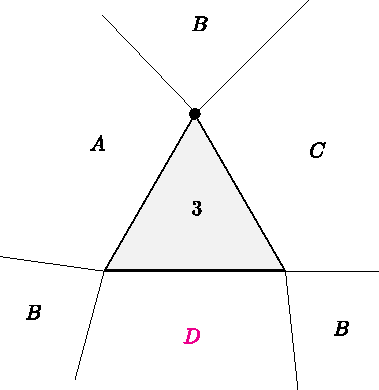
\includegraphics[scale=1]{fig/22.pdf}
	%\caption{}
\end{figure}

But extending to multiple vertices, we arrive at a contradiction: neither $A$ nor $C$ can occupy the pink face while making all vertices identical.

\newpage

% ------------------------------
% 5.23
% ------------------------------
\begin{exer}[5.23]
4 faces per vertex. If two triangles, they can't be adjacent; the other two faces must also be identical.
\end{exer}

\textbf{First part:} Suppose the two triangles are adjacent, then we have the situation below.

\begin{figure}[H]
	\centering
	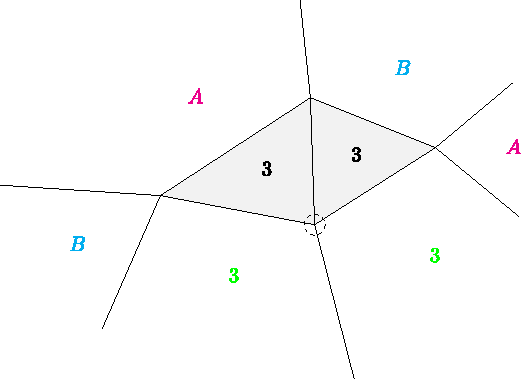
\includegraphics[scale=1]{fig/23.pdf}
	%\caption{}
\end{figure}

Since each vertex must be identical, the blue (pink) faces are taken up by another face $A$ ($B$). But then since each vertex has two adjacent triangles touching it, both green faces are also triangles. But then the highlighted vertex is surrounded by only triangles, a contradiction.

\textbf{Second part:} Suppose $A \neq B$, then we get the following situation.

\begin{figure}[H]
	\centering
	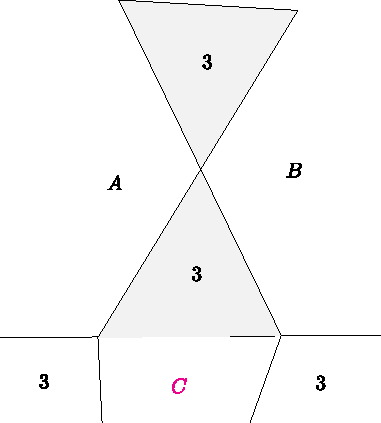
\includegraphics[scale=1]{fig/23b.pdf}
	%\caption{}
\end{figure}

But the pink face cannot be $A$ or $B$, as then not all the vertices would be identical. Thus $A = B$.

\newpage

% ------------------------------
% 5.25
% ------------------------------
\begin{exer}[5.25]
Classify the semiregular polyhedra with 3 faces per vertex.
\end{exer}

All possible semiregular polyhedra with three faces per vertex will have representation $(a,b,c)$; we have to find all valid $a,b,$ and $c$. First note that if $a$ is odd, then $b=c$. To see why, note that for all vertices to be identical, $b$ and $c$ must alternate around the face with $a$ edges, but this is not possible if $a$ is odd. This situation when $a=5$ is pictured below.

\begin{figure}[H]
	\centering
	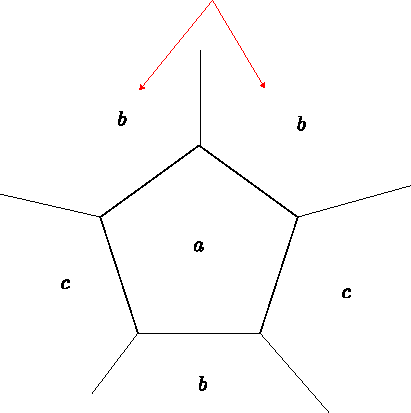
\includegraphics[scale=1]{fig/25.pdf}
	%\caption{}
\end{figure}

Using this same logic, we have that if $a$ is odd and $b$ is odd, then $a=b=c$. The only time $b=c$ and neither equals $a$ is when $b=c$ is even. Finally, we can eliminate all combinations of $a$ and $b=c$ whose angles add up to $\geq 360\degree$. This gives us the list
\[
	(3,3,3), \; (3,4,4), \; (3,6,6),\;(3,8,8),\;(3,10,10),\;(3,12,12),\\
	(5,5,5),\;(5,6,6).
\] 
Now suppose $a$ is even. We can apply the same reasoning about odds from before to conclude that $b$ and $c$ must also be even. Similar to above, we have
\[
	(4,4,4),\;(4,6,6),\;(4,8,8),\;(6,6,6).
\] We no longer have the restriction that $b=c$, though, so we can take all the triples with angle sums $\leq 360\degree$, giving
\[
	(4,4,n) \text{ for any } n,\; (4,6,8),\; (4,6,10),\; \text{ and } (4,6,12).
\] 

\newpage

% ------------------------------
% 5.26
% ------------------------------
\begin{exer}[5.26]
What are all the Euclidean tilings with five or six faces?
\end{exer}

\textbf{Five faces:} There are three possible tilings with five faces, since there are only three combinations of five polygons such that their angles add to exactly $360\degree$. They are
\[
	(3,3,3,3,6), (3,3,3,4,4), (3,3,4,3,4).
\] These are unique up to cyclic rotation. Any other combination of polygons give angles that don't sum to exactly $360\degree$.

\textbf{Six faces:} For six faces, the only tiling is $(3,3,3,3,3,3)$. Any other combination clearly gives an angle sum greater than $360\degree$, so any other combination of six polygons is neither a tiling nor a polyhedron.

\newpage

% ------------------------------
% 6.5
% ------------------------------
\begin{exer}[6.5]
Show that any quadrilateral's angles sum to $\leq 360\degree$.
\end{exer}

Take any quadrilateral $ABCD$ and decompose it into two triangles, as shown below.

\begin{figure}[H]
	\centering
	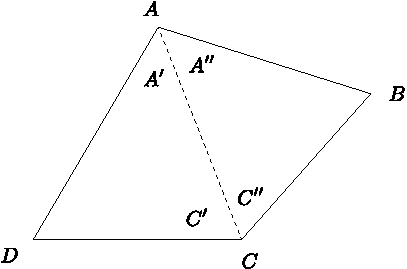
\includegraphics[scale=1]{fig/5.pdf}
	%\caption{}
\end{figure}

Since by Theorem 6.2 (which is true in \textit{any} geometry) the angles in a triangle sum to $\leq 180\degree$, we have
\[
	A + B+C+D = (A+A'+C')+(B+C''+A'') \leq 180\degree + 180\degree = 360\degree.
\] 

\newpage

% ------------------------------
% 6.7
% ------------------------------
\begin{exer}[6.7]
If a triangle's angles sum to 180, then there is a right triangle whose angles sum to 180. This means we can contruct a rectangle.
\end{exer}

Suppose $\Delta ABC$'s angles add up to $180\degree$. At least one of its altitudes must intersect one of its component lines, as depicted below.

\begin{figure}[H]
	\centering
	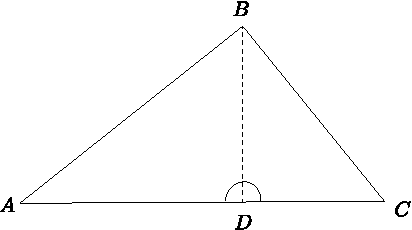
\includegraphics[scale=1]{fig/7.pdf}
	%\caption{}
\end{figure}

Note that we've added $180\degree$ worth of angles here since we added two right angles. Thus $A+B+C+D = 180\degree + 180\degree = 360\degree$. Now we know by Theorem 6.2 that the angles in a triangle are at most $180\degree$. But since the sums of the angles of the two triangles above give exactly $360\degree$, they must both sum to exactly $180\degree$.

Now take some right triangle $\Delta ABC$ with angles summing to $180\degree$ (which we just proved existed under our assumptions). Then assume, as shown below, that $C=90\degree$ and $A+B=90\degree$.

\begin{figure}[H]
	\centering
	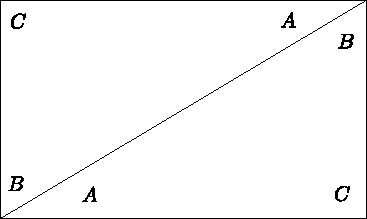
\includegraphics[scale=1]{fig/6b.pdf}
	%\caption{}
\end{figure}

Then copying $\Delta ABC$ and aligning the two triangles' hypotnuses with each other gives a rectangle since, as noted earlier, $C=B+C=90\degree$.

\newpage

% ------------------------------
% 6.16
% ------------------------------
\begin{exer}[6.16]
For any $\varepsilon> 0$, there's an $R$ on $QM$ such that $\angle PRQ < \varepsilon$.
\end{exer}

Fix $\varepsilon>0$. Now construct a sequence of triangles as follows: Start with right angle $\angle PQM$, then mark the point $R_0$ on $QM$ that is distance $|PQ|$ from $Q$.

\begin{figure}[H]
	\centering
	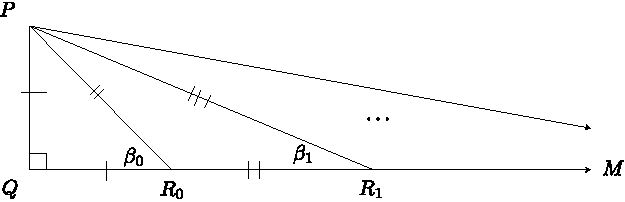
\includegraphics[scale=1]{fig/16.pdf}
	%\caption{}
\end{figure}

Now find the point on $QM$ that is $|PR_0|$ to the right of $R_0$, and use this to form another triangle with bottom angle $\beta_2$. Now continue inductively to define a sequence of angles $\left\{ \beta_n \right\}_{n \in \mathbb{N}_{0}}$.

Note since $PQR_0$ is isosceles, $\beta_0 =45\degree$. Then its complement is $(180-45)\degree$, so $PR_0R_1$ being isosceles implies $\beta_1 = \frac{45}{2}\degree$. In general, $\beta_{n} = \frac{45}{2^{n}}\degree$. Then if $N > \log_2(45/\varepsilon)$, we have
\[
	\beta_N = \frac{45}{2^{N}}\degree < \frac{45}{(45/\varepsilon)} \degree \varepsilon.
\] Choose any such $N$, then $R_{N}$ satisfies the problem statement.

\newpage

\end{document}
